\iffalse
\documentclass[12pt]{article}
\usepackage{graphicx}
\usepackage[none]{hyphenat}
\usepackage{graphicx}
\usepackage{listings}
\usepackage[english]{babel}
\usepackage{graphicx}
\usepackage{caption} 
\usepackage{booktabs}
\usepackage{array}
\usepackage{amssymb} % for \because
\usepackage{amsmath}   % for having text in math mode
\usepackage{extarrows} % for Row operations arrows
\usepackage{listings}
\lstset{
  frame=single,
  breaklines=true
}
\usepackage{hyperref}
  
%Following 2 lines were added to remove the blank page at the beginning
\usepackage{atbegshi}% http://ctan.org/pkg/atbegshi
\AtBeginDocument{\AtBeginShipoutNext{\AtBeginShipoutDiscard}}
\usepackage{gensymb}


%New macro definitions
\newcommand{\mydet}[1]{\ensuremath{\begin{vmatrix}#1\end{vmatrix}}}
\providecommand{\brak}[1]{\ensuremath{\left(#1\right)}}
\providecommand{\sbrak}[1]{\ensuremath{{}\left[#1\right]}}
\providecommand{\norm}[1]{\left\lVert#1\right\rVert}
\providecommand{\abs}[1]{\left\vert#1\right\vert}
\newcommand{\solution}{\noindent \textbf{Solution: }}
\newcommand{\myvec}[1]{\ensuremath{\begin{pmatrix}#1\end{pmatrix}}}
\let\vec\mathbf


\begin{document}

\begin{center}
\title{\textbf{Convex Optimization}}
\date{\vspace{-5ex}} %Not to print date automatically
\maketitle
\end{center}
\setcounter{page}{1}

\section{11$^{th}$ Maths - Chapter 10}
This is Problem-3.1 from Exercise 10.3 
\begin{enumerate}

\solution 
\fi
Let $\vec{O}$ be the point from where we have to find the perpendicular distance and $\vec{P}$ be the foot of the perpendicular. The optimization problem can be expressed as
\begin{align}
	\label{eq:11/10/3/3/1/conv/Eq3}
	  \min_{\vec{x}} \norm{\vec{x}-\vec{O}}^2\\
	 \text{s.t.} \quad \vec{n}^T\vec{x} = c 
\end{align}
where 
\begin{align}
	\vec{n} = \myvec{-1 \\ \sqrt{3}},\,c = 8
\end{align}
The line equation can be expressed as
\begin{align}
	\label{eq:11/10/3/3/1/conv/Eq2}
	\vec{x} = \vec{A}+\lambda\vec{m}
\end{align}
where
\begin{align}
	\label{eq:11/10/3/3/1/conv/Eq1}
	\vec{m} = \myvec{1 \\ \frac{1}{\sqrt{3}}},\,
	\vec{A} = \myvec{-8 \\ 0}
\end{align}
\begin{enumerate}
\item Using the parameric form,
Substituting \eqref{eq:11/10/3/3/1/conv/Eq2} in \eqref{eq:11/10/3/3/1/conv/Eq3}, the optimization problem becomes
\begin{align}
	\min_{\lambda} \norm{ \lambda\vec{m} +\brak{\vec{A}-\vec{O}}}^2\\
	\implies \min_{\lambda}f\brak{\lambda} 	
	= \lambda^2\norm{\vec{m}}^2+ 2\lambda\brak{\vec{A}-\vec{O}}^\top\vec{m}+ + \norm{\vec{A}-\vec{O}}^2  
\label{eq:11/10/3/3/1/conv/Eq4}
\end{align}
$\because$ the coefficient of $\lambda^2> 0$, \eqref{eq:11/10/3/3/1/conv/Eq4} is a convex function.
Thus,
\begin{align}
	f^{\prime\prime}\brak{\lambda} &= 2\norm{\vec{m}}^2 \\ 
	\because f^{\prime\prime}\brak{\lambda} > 0, f^\prime\brak{\lambda_{min}} &= 0, \text{ for } \lambda_{min}
\end{align}
yielding
\begin{align}
	& f^\prime\brak{\lambda_{min}} =  2\lambda_{min}\norm{\vec{m}}^2 + 2\brak{\vec{A}-\vec{O}}^\top\vec{m}  = 0 \\
	\label{eq:11/10/3/3/1/conv/EqMin}
	\lambda_{min} &= -\frac{\brak{\vec{A}-\vec{O}}^\top\vec{m}}{\norm{\vec{m}}^2} 
\end{align}
We choose  
\begin{align}
	\vec{O} &= \myvec{ 0 \\ 0}
\end{align}
Substituting the values of $\vec{A}$, $\vec{O}$ and $\vec{m}$ in equation \eqref{eq:11/10/3/3/1/conv/EqMin}
\begin{align}
	\lambda_{min} &= -\frac{\brak{\myvec{-8 \\ 0 }-\myvec{0 \\ 0}}^\top\myvec{1 \\ \frac{1}{\sqrt{3}}}}{\norm{\myvec{1 \\ \frac{1}{\sqrt{3}}}}^2}\\ 
	&= 6
\end{align}
Substituring this value in equation \eqref{eq:11/10/3/3/1/conv/Eq2}
\begin{align}
	\vec{x}_{min} &= \vec{P} = \myvec{-8 \\ 0}+6\myvec{1 \\ \frac{1}{\sqrt{3}}}  \\
	&= \myvec{-2 \\ 2\sqrt{3}} \\
	OP &= \norm{\vec{P}-\vec{O}}^2 \\ 
	&  = 4
\end{align}
\item Solving using cvxpy, with 
\begin{align}
	&\vec{n} = \myvec{1 \\ -\sqrt{3}} \\
	&\vec{O} = \myvec{0 \\ 0} \\
	&c = -8 \\
	\label{eq:11/10/3/3/1/conv/minval}
	&  \min_{\vec{x}} \norm{\vec{x}-\vec{O}}^2 = 4, 
	 \vec{x}_{min} = \myvec{-2  \\ 3.46 } 
\end{align}
\end{enumerate}
The relevant figures are shown in \ref{fig:11/10/3/3/1/conv/Fig1} and \ref{fig:11/10/3/3/1/conv/Fig2}
\begin{figure}[!h]
	\begin{center}
		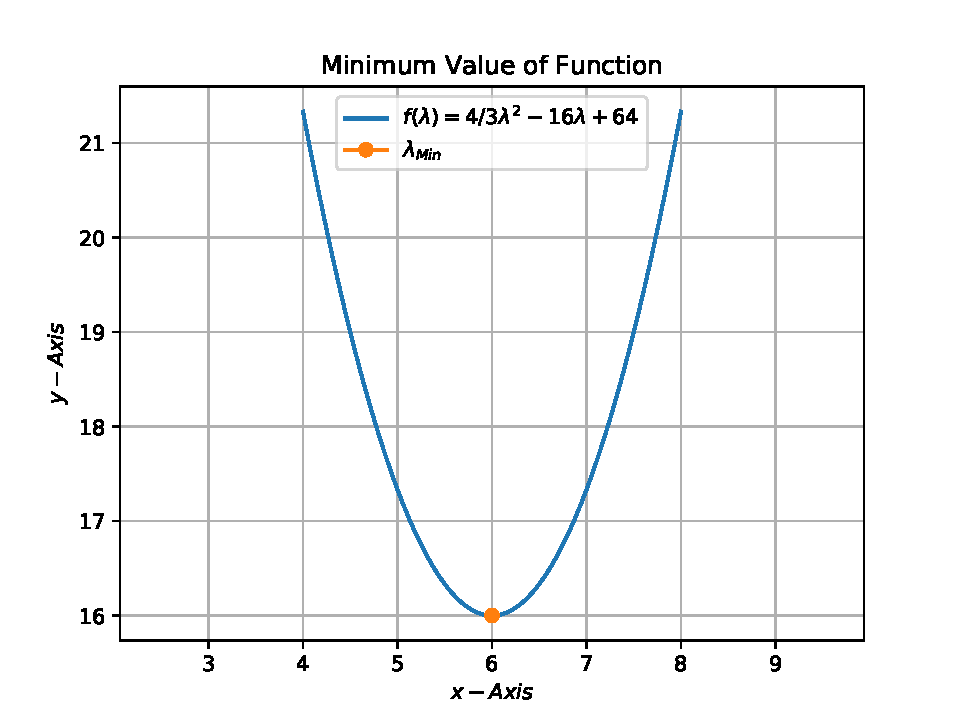
\includegraphics[width=\columnwidth]{11/10/3/3/1/conv/figs/problem3.1a.pdf}
	\end{center}
\caption{}
\label{fig:11/10/3/3/1/conv/Fig1}
\end{figure}
\begin{figure}[!h]
	\begin{center}
		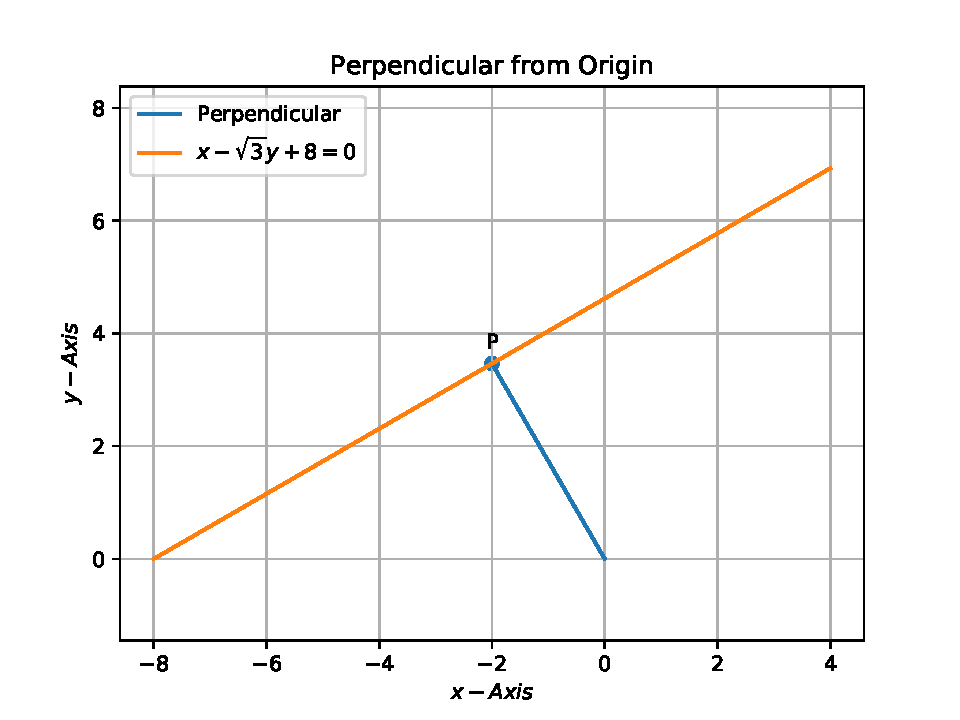
\includegraphics[width=\columnwidth]{11/10/3/3/1/conv/figs/problem3.1b.pdf}
	\end{center}
\caption{}
\label{fig:11/10/3/3/1/conv/Fig2}
\end{figure}
